\section*{The Probabilistic Framework}
Our solution is based on discrete \emph{Markov processes}, which are a special case of stochastic processes. For a Markov process, the next state depends only on the present state and not on past states.

An example of a discrete Markov process is that of throwing dice and summing the results: the throws and state space are discrete, and the possible states (sums) after the next throw depends only on the current state.

In mathematical terms, a discrete Markov process satisfies the following:
\begin{equation}
 p\left(Z_{n+1}|Z_n \wedge Z_{n-1} \wedge Z_{n-2} \wedge \dots \wedge Z_0\right) = p\left(Z_{n+1}|Z_n\right),
\end{equation}
where $Z_n$ is the system's \emph{state} after step $n$ and $p\left(Z_{n+1}|Z_n, Z_{n-1}, Z_{n-2}, \dots, Z_0\right)$ is the probability that the system will have state $Z_{n+1}$ in the next step, given that the previous states where $Z_n, Z_{n-1}, Z_{n-2}, \dots, Z_0$.

A \emph{hidden Markov model} (HMM) describes a Markov process where one cannot measure the state $Z$ of the system directly - it is ``hidden''. Instead we obtain an \emph{observation} $I$\footnote{In this project, the observation is a grayscale \emph{image}, which is why we use the symbol $I$.}  of the state. This \emph{perception} is generally non-deterministic, so we need to denote it as $p(I_n|Z_n)$ which is the probability that we will observe $I_n$ if the current state of the system is $Z_n$.

\subsection*{The Particle Filter}
The Particle Filter is a technique for simulating a process described by a HMM. It uses a finite set $X_{n+1}$ of hypotheses to approximate the probability function $\cprobnext{Z}$. The hypotheses $X_n$ are also known as \emph{particles}, thereby the term ``particle filter''.

\begin{figure}
  \centering
  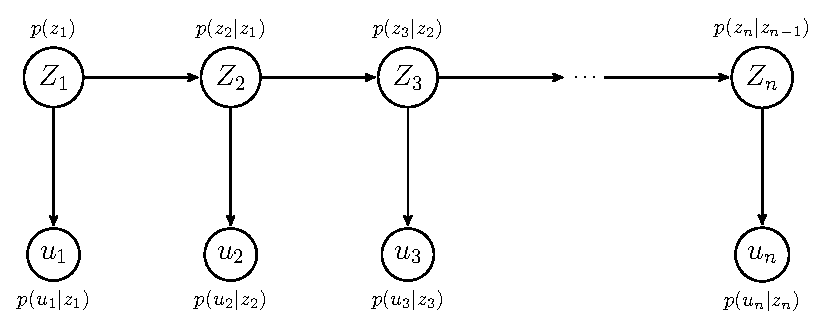
\includegraphics[width=\textwidth]{hmm-graph.pdf}
  \caption{Schematic image of the Particle Filter working alongside a Hidden Markov Model.}
  \label{fig:hmm-graph}
\end{figure}

Figure \ref{fig:hmm-graph} shows the working principle of the Particle Filter working alongside a Hidden Markov Model. The following is the core function of the Particle Filter:

\begin{quote}
  \emph{The particle filter attempts to approximate the probability density function $\cprobnext{Z}$ as a set $X_{n+1}$ of discrete hypotheses.}
\end{quote}

More particles mean greater accuracy, since the PDF can then be approximated more closely. However, using many particles is also computationally expensive. Therefore the number of particles is an important quantity. The Particle Filter employs a few tricks to \emph{filter} the hypotheses, keeping probable ones and throwing improbable ones away, in order to reduce the number of particles needed for a good approximation. The following is a quick run-down of how the Particle Filter does this. For brevity, we will commit some abuse of notation.

\begin{description}
\item[Initialization:] Since the algorithm only does tracking, we need to initialize the algorithm with a start guess $x_0$. Using this we take a number of samples $X_0 \sim \ndist{x_0}{\Sigma}$ and let the set $X_0$ be an approximation of $\prob{Z_0}$ \footnote{The problem of initialization is a tricky one\cite{Hedvig}, and is not covered in this project. In our testing implementation, we used $\Sigma = 0$}.
\item[Prediction:] The hypotheses $X_n$ are updated in the \emph{prediction} step to an approximation of $\cprobnext{Z}_{n+1}$. This is done by drawing new samples $\bar{X}_{n+1} \sim \cprobnext{X}$.
\item[Perception:] By measuring the state of the system, we gain an \emph{observation} $I_{n+1} \sim \cprob{I_{n+1}}{Z_{n+1}}$ of the state $Z_{n+1}$.
\item[Filtering:] The observation $I_{n+1}$ of the system is then used for filtering bad hypotheses out of $\bar{X}_{n+1}$. We draw samples $X_{n+1}$ from $\bar{X}_{n+1}$ with probabilities given by $\cprob{I_{n+1}}{\bar{X}_{n+1}}$. As a result, $X_{n+1}$ will be a subset of $\bar{X}_{n+1}$ where more probable hypotheses appear multiple times. For this reason, this is also known as the \emph{resampling} step. The set $X_{n+1}$ is the \emph{belief}, our approximation of $\cprobnext{Z}$.
\item[Selection:] Finally, we produce a single hypothesis $x_{n+1}$ from $X_{n+1}$ as our \emph{estimate} of the state $Z_{n+1}$. Supposing $X_{n+1}$ is a good approximation of $\cprobnext{Z}$, and that $\cprobnext{Z}$ is unimodal, the mean value of $X_{n+1}$ is a good hypothesis since it approximates the expectation of $\cprobnext{Z}$.
\end{description}


\subsection*{Implementing the Particle Filter}
An implementation of the Particle Filter consists mainly of designing the probability functions $\cprobnext{X}$ and $\cprob{I_n}{X_n}$, and providing the algorithm with a sensible initialization. This is what this project is all about. The rest just consists of taking samples from these functions.
